\centerline{\bf \Huge }
\centerline{\bf \Huge }

\begin{flushright}
        \scriptsize{}
\end{flushright}

\problem{1}
Решите уравнение $x+\sqrt{3+\sqrt{x}}=3$.

\textbf{Решение:}

Если $x>1$, то выражение слева больше 3. Если $0 \leqslant x<1$, то выражение слева меньше 3. Остается единственный вариант $x=1$, который нам подходит.

\problem{2}
Решите уравнение $x^4 + 4x^3 + 6x^2 + 4x + 1 = 0$.

\textbf{Решение:}

Очевидно, что $0$ не является решением уравнения, поэтому поделим обе части на $x^2$.

$$
x^2 + 4x + 6 + 4 \cdot \dfrac{1}{x} + \dfrac{1}{x^2} = 0
$$

Напрашивается замена $x + \dfrac{1}{x} = t$. Почему? Да потому что $x^2 + \dfrac{1}{x^2} = t^2 - 2$ и наше уравнение перепишется в виде:

$(t^2 - 2) + 4t + 6 = 0$.

Теперь дважды решаем квадратное уравнение и получаем, что исходное уравнение имеет корень -1 причём кратности 4. Внимательные ученики могли сразу заметить, что коэффициенты нашего многочлена это биномиальные коэффициенты с основанием 4. Отсюда сразу ответ $(x+1)^4$. Вообще говоря, замена $t = x + \dfrac{1}{x}$ не случайна. Она происходит в уравнениях, где коэффициенты многочлена образуют палиндром. Такие уравнения называются $\textit{возвратными}.$

\problem{3}


\problem{4}


\problem{5}
Решите неравенство $\dfrac{\sqrt{\left(x^2-81\right)\left(x^2+10 x+25\right)}}{\left(169-x^2\right)\left(x^2+12 x+11\right)} \leqslant 0$.

\textbf{Решение:}

$$
\begin{aligned}
& \frac{\sqrt{\left(x^2-81\right)\left(x^2+10 x+25\right)}}{\left(169-x^2\right)\left(x^2+12 x+11\right)} \leqslant 0 \\
& \frac{\sqrt{(x-9)(x+9)(x+5)^2}}{(13-x)(13+x)(x+1)(x+11)} \leqslant 0 .
\end{aligned}
$$


Поменяем знак неравенства, чтобы во всех скобках коэффициенты при $\boldsymbol{x}$ были положительны:

$$
\frac{\sqrt{(x-9)(x+9)(x+5)^2}}{(x-13)(x+13)(x+1)(x+11)} \geqslant 0 .
$$


С учетом ОДЗ неравенства рассмотрим два случая: когда подкоренное выражение равно нулю и когда оно положительно. Неравенство перепишется в виде следующей эквивалентной совокупности:

$$
\left[\begin{array}{l}
\left\{\begin{array}{l}
(x-9)(x+9)(x+5)^2>0 \\
(x-13)(x+13)(x+1)(x+11)>0
\end{array}\right. \\
\left\{\begin{array}{l}
(x-9)(x+9)(x+5)^2=0 \\
(x-13)(x+13)(x+1)(x+11) \neq 0
\end{array}\right.
\end{array}\right.
$$


Вторая система из этой совокупности задаёт просто набор точек:

$$
\left[\begin{array}{l}
\left\{\begin{array}{l}
(x-9)(x+9)(x+5)^2>0 \\
(x-13)(x+13)(x+1)(x+11)>0
\end{array}\right. \\
x=9 \\
x=-9 \\
x=-5
\end{array}\right.
$$


Решение первой системы изобразим на координатных осях:


\begin{center}
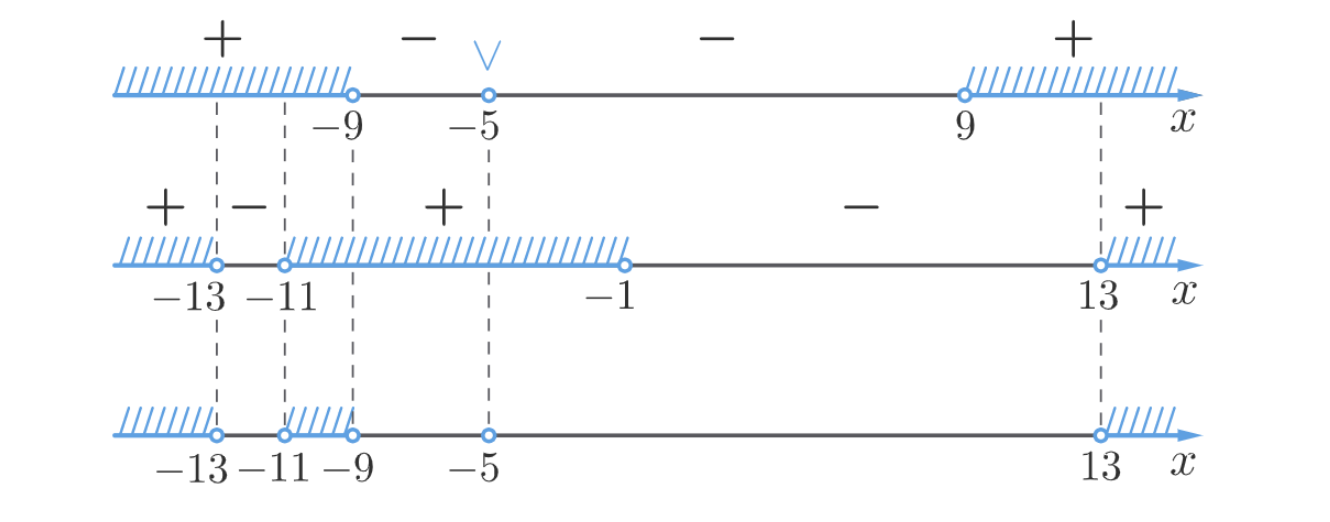
\includegraphics[width=1\textwidth]{АА/ЕМ/9 лицей/ineq.png}
\end{center}

Учтем точки из набора и запишем ответ.

Ответ: $(-\infty ;-13) \cup(-11 ;-9] \cup\{-5 ; 9\} \cup(13 ;+\infty)$.

\problem{6}
Найдите все значения параметра $a$, при каждом из которых неравенство

$$
\left(x^2-(a+8) x-6 a^2+24 a\right) \sqrt{3-x} \leqslant 0
$$

имеет единственное решение.


\newpage

\hspace{3mm}

\textbf{Решение:}

Заметим, что значение $x=3$ является решением неравенства при любых значениях параметра. Значит, других решений быть не должно: при $3-x>0$ первая скобка должна быть положительной.
Рассмотрим уравнение $x^2-(a+8) x-6 a^2+24 a=0$. Его дискриминант равен $D=(a+8)^2-4\left(-6 a^2+24 a\right)=25 a^2-80 a+64=(5 a-8)^2$. Из неотрицательности дискриминанта следует, что соответствующая квадратичная функция (первая скобка) принимает неположительные значения на отрезке между корнями (или только в вершине, если корень один). Нам требуется, чтобы при $x<3$ эта первая скобка принимала только положительные значения, то есть первая скобка может быть неположительной только при $x \geqslant 3$, значит, меньший корень должен лежать не левее, чем 3:

$$
\begin{gathered}
\dfrac{a+8-|5 a-8|}{2} \geqslant 3 \quad \Longleftrightarrow \quad a+2 \geqslant|5 a-8| \\
-a-2 \leqslant 5 a-8 \leqslant a+2 \Longleftrightarrow 1 \leqslant a \leqslant \dfrac{5}{2}
\end{gathered}
$$


Ответ: $\left[1 ; \dfrac{5}{2}\right]$


\problem{7}
Анджур с друзьями решили устроить пикник. Для этого им от пункта А нужно добраться вниз по реке до пункта В, причем в их распоряжении есть два катера. Считая себя самым ответственным, Анджур вызвался самостоятельно доехать до пункта В на более быстроходном катере и начать готовить место для пикника. Оба катера вышли одновременно из пункта A. Однако, промчавшись восемь километров, Анджур заметил на берегу машущего ему рукой Расула, который просил по старой дружбе довезти его до пункта С. И хоть пункт С Анджур уже проехал, он согласился. По пути в пункт С Анджур с Расулом встретили идущий навстречу второй катер с друзьями Анджура, откуда те крикнули, что им до пункта В осталась треть пути и чтобы Анджур нигде не задерживался. Доставив Расула в пункт С, Анджур немедленно помчался догонять друзей. Найдите расстояние между пунктами В и С, если известно, что оба катера пришли в пункт В одновременно, скорости катеров постоянны, а Анджур, действительно, нигде не задерживался.

\textbf{Решение:}

Рассмотрим график движения, где по $ADCB$ двигался первый катер, а по $AB$ --- второй

 \begin{center}
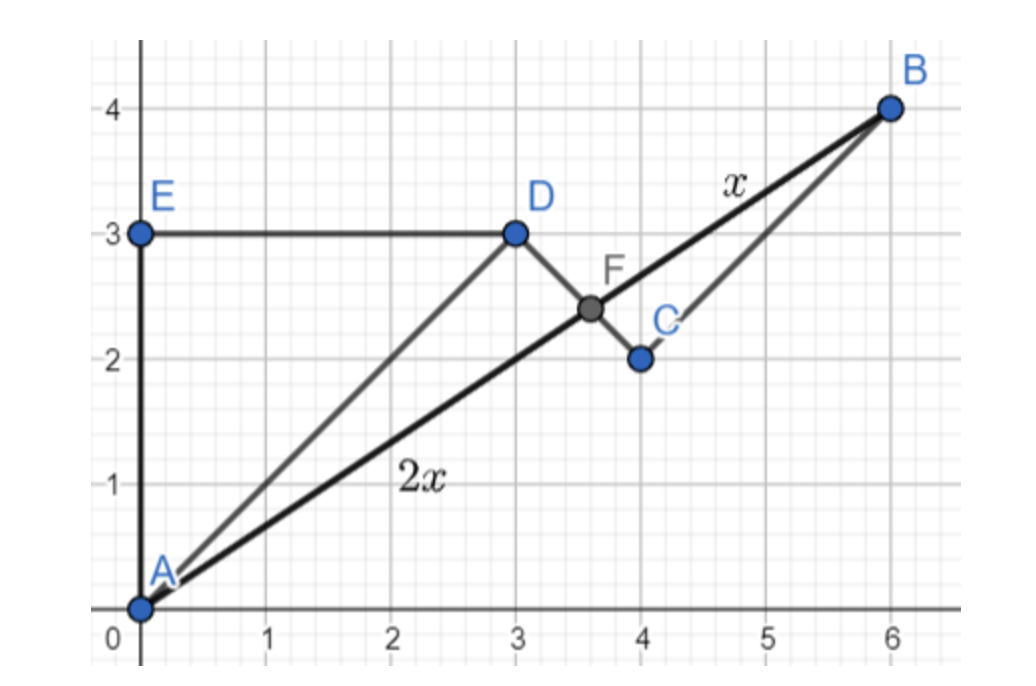
\includegraphics[width=0.8\textwidth]{АА/ЕМ/9 лицей/movement.png}
\end{center}

Здесь $A E=8$ из условия, $A D$ и $B C$ параллельны (тангенсы их углов наклона к оси равны скорости катера вниз по реке), откуда $\triangle A D F \sim \triangle B C F$ с коэффициентом $2: 1(\angle A D F=\angle F C B)$, откуда на отрезке $C B$ первый катер прошёл 4 км.

\problem{8}
Разложите на множители выражение $(a + b + c)^3 - a^3 - b^3 - c^3$

\textbf{Решение:}
При $a=-b$ многочлен обращается в ноль, значит, по теореме Безу он делится на $a+b$. Аналогично он делится на $a+c$ и $b+c$. Учитывая степень многочлена он равен $k(b+c)(a+b)(a+c)$. Подставляя $a=b=c=1$, находим коэффициент $k$.

Ответ: $3(b+c)(a+b)(a+c)$.

\problem{9}
Аркадий Владимирович написал на доске уравнение вида  $x^2 + px + q = 0$  с целыми ненулевыми коэффициентами $p$ и $q$. Временами к доске подходили ученики 9в класса, стирали уравнение, после чего составляли и записывали уравнение такого же вида, корнями которого являются коэффициенты стёртого уравнения. В какой-то момент составленное уравнение совпало с тем, что было написано на доске изначально. Какое уравнение изначально было написано на доске?

\textbf{Решение:}

По теореме Виета, коэффициенты нового трёхчлена равны - $(p+q)$ и $p q$ соответственно. Заметим, что ни у одного из написанных трёхчленов второй коэффициент (при $x$ ) не может быть равен нулю. Действительно, в этом случае у всех последующих трёхчленов свободный член был бы равен нулю, а значит, среди них не мог встретиться исходный многочлен. Далее, у каждого следующего трёхчлена модуль свободного члена не меньше, чем у предыдущего. Следовательно, модули всех свободных членов равны, а значит, все вторые коэффициенты равны $\pm 1$. Итак, $-(p+q)= \pm 1, p= \pm 1$. Поэтому для первого трёхчлена возможны только два варианта: $x^2+x-2$ и $x^2-x+2$. Несложно проверить, что в первом случае трёхчлен не изменяется, а во втором сначала получается трёхчлен $x^2-x-2$, а потом - трёхчлен $x^2+3 x+2$, модуль второго коэффициента которого не равен единице.

Ответ: $x^2+x-2$